\documentclass[a4paper,10pt]{article}

\usepackage[utf8]{inputenc}
\usepackage{graphicx}
\usepackage{fancybox}
\usepackage{verbatim}
\newcommand{\HRule}{\rule{\linewidth}{0.5mm}}

\begin{document}

\begin{titlepage}

\begin{center}


% Upper part of the page


\textsc{\LARGE Simulación de Sistemas 72.25}\\[1.5cm]

\textsc{\Large Simulación de un Centro de Mantenimiento para Unidades de Transporte de Pasajeros}\\[0.5cm]


% Title
\HRule \\[0.4cm]
{ \huge \bfseries Trabajo Práctico Final}\\[0.4cm]

\HRule \\[1.5cm]

% Author and supervisor
\begin{minipage}{0.4\textwidth}
\begin{flushleft} \large
\emph{Authors:}\\
Alberto Miguel \textsc{Pose}\\
Juan Ignacio \textsc{Catalano}\\
Martín \textsc{Palombo}\\
Santiago José \textsc{Vazquez}\\
\end{flushleft}
\end{minipage}

\vfill

\end{center}
\thispagestyle{empty}
\end{titlepage}


\section{Punto (a)}
Se modelaron los intervalos de tiempos entre arribos y el tiempo de servicio de ER a partir de los datos provistos en los archivos históricos \verb|arriboscop| y \verb|ercop| respectivamente. Para ello, se graficaron los histogramas correspondientes. En la Figura \ref{fig:hist_arriboscop} vemos el histograma correspondiente a los intervalos de tiempos entre arribos. Para la elección de los intervalos de clase se utilizó el criterio de Nuñez. Como podemos ver intuitivamente, la distribución de los datos en este caso es una exponencial. En la Figura \ref{fig:hist_servicios} podemos ver el histograma correspondiente a los tiempos de servicios de ER. De nuevo, intuitivamente podemos ver que la distribución en este caso es una normal. Además, el simulado es un tipo proceso que generalmente tiene distribución de ese tipo. Esto nos sirve para reforzar nuestra hipótesis.

\begin{figure}[ht]
\begin{center}
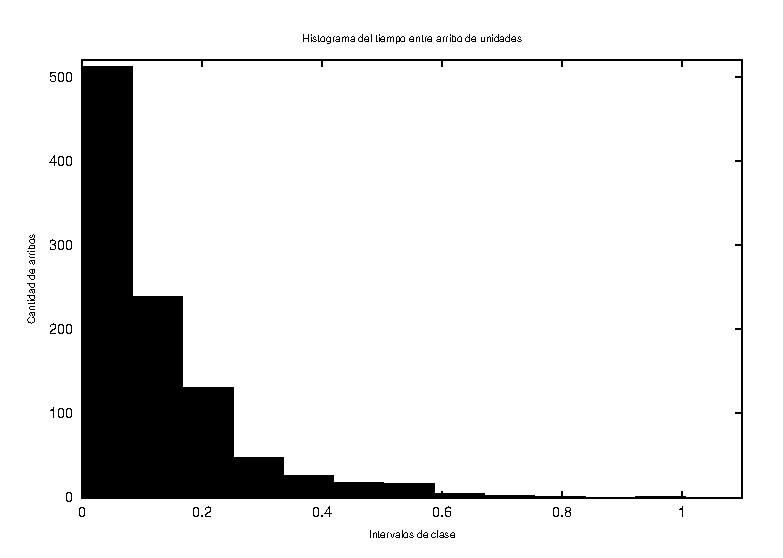
\includegraphics[width=12cm]{../src/parteA/hist_arribos.eps}
\caption{\label{fig:hist_arriboscop} Histograma correspondiente a los intervalos de tiempos entre arribos.}
\end{center}
\end{figure}

\begin{figure}[ht]
\begin{center}
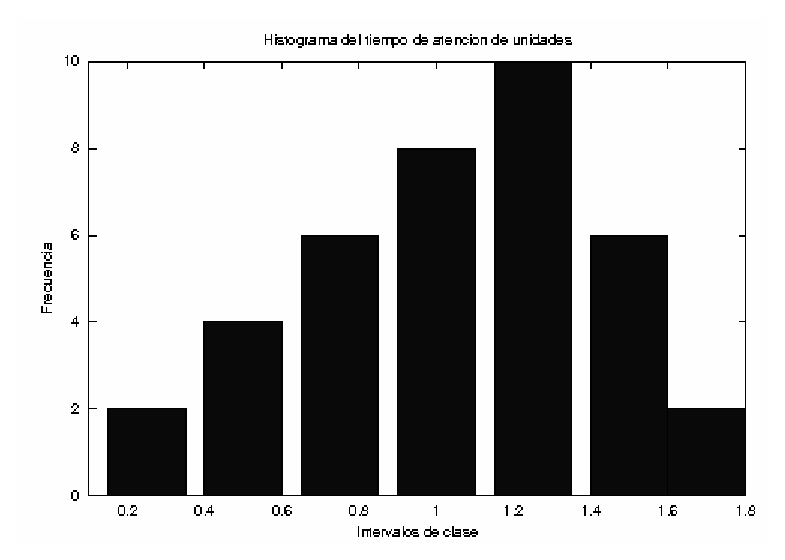
\includegraphics[width=12cm]{../src/parteA/hist_servicios.eps}
\caption{\label{fig:hist_servicios} Histograma correspondiente a los tiempos de servicios de ER.}
\end{center}
\end{figure}

Se utilizaron los test de  $\chi^2$ y el Gráfico QQ para verificar que las distribuciones son las indicadas previamente. La tabla corresponde al test realizado para verificar la distribución exponencial de los tiempos entre arribos, se ve en la Tabla \ref{tab:chi_table}. El test $\chi^2$ arrojó un valor de $18.213$ que implica un nivel de significación de $5\%$. 
%Para el de KS, obtuvimos un valor de $0.99966$. Se verifica la distribución ya que es mayor a $0.375$, que es el valor obtenido de tabla para un nivel de significación como el especificado anteriormente y 12 intervalos.

\begin{table}[ht]
\begin{center}
\begin{tabular}{l*{6}{c}r}
\hline
Clase& $O_i$ & $E_i$  & $O_i - E_i$ & $(O_i - E_i)^2$ & $\frac{(O_i - E_i)^2}{E_i}$\\
\hline
1&512.000000&483.209027&-28.790973&828.920123&1.715448\\
2&239.000000&249.533949&10.533949&110.964084&0.444685\\
3&131.000000&128.861814&-2.138186&4.571839&0.035479\\
4&48.000000&66.545523&18.545523&343.936416&5.168438\\
5&26.000000&34.364770&8.364770&69.969378&2.036079\\
6&18.000000&17.746309&-0.253691&0.064359&0.003627\\
7&17.000000&9.164371&-7.835629&61.397088&6.699542\\
8&5.000000&4.732572&-0.267428&0.071518&0.015112\\
9&2.000000&2.443947&0.443947&0.197089&0.080644\\
10&1.000000&1.262079&0.262079&0.068685&0.054422\\
11&0.000000&0.651750&0.651750&0.424778&0.651750\\
12&1.000000&0.336570&-0.663430&0.440139&1.307719\\
\hline
\end{tabular}
\caption{\label{tab:chi_table} Cómputos para el test $\chi^2$ para la distribución exponencial.}
\end{center}
\end{table}

%\begin{table}[ht]
%\begin{center}
%\begin{tabular}{l|l*{12}{c}r}
%\hline
%$x_i$&0.512000&0.239000&0.131000&0.048000&0.026000&0.018000\\
%$i/n$&0.483764&0.733585&0.862594&0.929216&0.963621&0.981387\\
%$\frac{i}{n} - x_i$&-0.028236&0.494585&0.731594&0.881216&0.937621&0.963387\\
%$x_i - \frac{i-1}{n}$&0.512000&0.155667&-0.035667&-0.202000&-0.307333&-0.398667\\
%\hline
%\end{tabular}
%\caption{\label{tab:ks_table_first} Cómputos para el test $KS$. Intervalos del 1 al 6. Para la distribución exponencial}
%\end{center}
%\end{table}

%\begin{table}[ht]
%\begin{center}
%\begin{tabular}{l|l*{12}{c}r}
%\hline
%$x_i$&0.017000&0.005000&0.002000&0.001000&0.000000&0.001000\\
%$i/n$&0.990562&0.995300&0.997747&0.999011&0.999663&1.000000\\
%$\frac{i}{n} - x_i$&0.973562&0.990300&0.995747&0.998011&0.999663&0.999000\\
%$x_i - \frac{i-1}{n}$&-0.483000&-0.578333&-0.664667&-0.749000&-0.833333&-0.915667\\
%\hline
%\end{tabular}
%\caption{\label{tab:ks_table_second} Cómputos para el test $KS$. Intervalos del 7 al 12. Para la distribución exponencial}
%\end{center}
%\end{table}

Además, se utilizó el test de $\chi^2$ para verificar la distribución normal de los tiempos de servicio de ER. Las tablas correspondientes a los tests realizados para verificar la distribución normal de los tiempos de servicios de ER, se ven en las Tablas \ref{tab:chi_table_norm} y \ref{tab:ks_table_norm}. El test $\chi^2$ arrojó un valor de $1.56995$ que implica un nivel de significación de $5\%$. Para el de KS, obtuvimos un valor de 0.94737. Se verifica la distribución ya que es mayor a $0.486$, que es el valor obtenido de tabla para un nivel de significación de 0.05 y 7 intervalos.


\begin{table}[ht]
\begin{center}
\begin{tabular}{l*{6}{c}r}
\hline
Clase& $O_i$ & $E_i$  & $O_i - E_i$ & $(O_i - E_i)^2$ & $\frac{(O_i - E_i)^2}{E_i}$\\
\hline
1&2.000000&1.210939&-0.789061&0.622618&0.514161\\
2&4.000000&3.619368&-0.380632&0.144881&0.040029\\
3&6.000000&7.209408&1.209408&1.462667&0.202883\\
4&8.000000&9.574088&1.574088&2.477754&0.258798\\
5&10.000000&8.478138&-1.521862&2.316063&0.273181\\
6&6.000000&5.005838&-0.994162&0.988358&0.197441\\
7&2.000000&2.452396&0.452396&0.204662&0.083454\\
\hline
\end{tabular}
\caption{\label{tab:chi_table_norm} Cómputos para el test $\chi^2$ para la distribución normal.}
\end{center}
\end{table}

\begin{table}[ht]
\begin{center}
\begin{tabular}{l|l*{12}{c}r}
\hline
$x_i$&0.052632&0.105263&0.157895&0.210526&0.263158&0.157895&0.052632\\
$i/n$&0.032249&0.128636&0.320630&0.575598&0.801380&0.934690&1.000000\\
$\frac{i}{n} - x_i$&-0.020383&0.023373&0.162735&0.365072&0.538222&0.776795&0.947368\\
$x_i - \frac{i-1}{n}$&0.052632&-0.037594&-0.127820&-0.218045&-0.308271&-0.556391&-0.804511\\
\hline
\end{tabular}
\caption{\label{tab:ks_table_norm} Cómputos para el test $KS$. Para la distribución normal}
\end{center}
\end{table}

\section{Punto (b)}
Las colas del sistema se denominan como se muestra en la Figura \ref{fig:events_diagram}. Como podemos ver, quedan
determinadas por el conjunto 
\[
S = \{UI, ER1, ER2, ER3, ST\}
\]
El estado del sistema se encuentra compuesto por la longitud y el estado de servicio (busy/free) de cada una de las 3 colas. Las características del sistema, determinan que todas las colas se modelan como de capacidad infinita y utilizan la disciplina FIFO (First In First Out).

\section{Punto (c)}
Los eventos de nuestro sistema quedan definidos por las llegadas y partidas de una UI a cada una de las etapas del proceso de mantenimiento. Como podemos ver en la Figura \ref{fig:events_diagram}, los tipos de eventos estan dados por el conjunto
\[
 E = \{IUI, OUI, IER, OER, IST, OST\}
\]
Como asumimos que la salida de una sección y paso a la próxima se realiza instantaneamente, podemos unificar los tipos de eventos $OUI$ con $IER$ y $OER$ con $IST$. Por lo tanto $E$ nos queda reducido a
\[
 E = \{IUI, IER, IST, OST\}
\]

\begin{figure}[ht]
\begin{center}
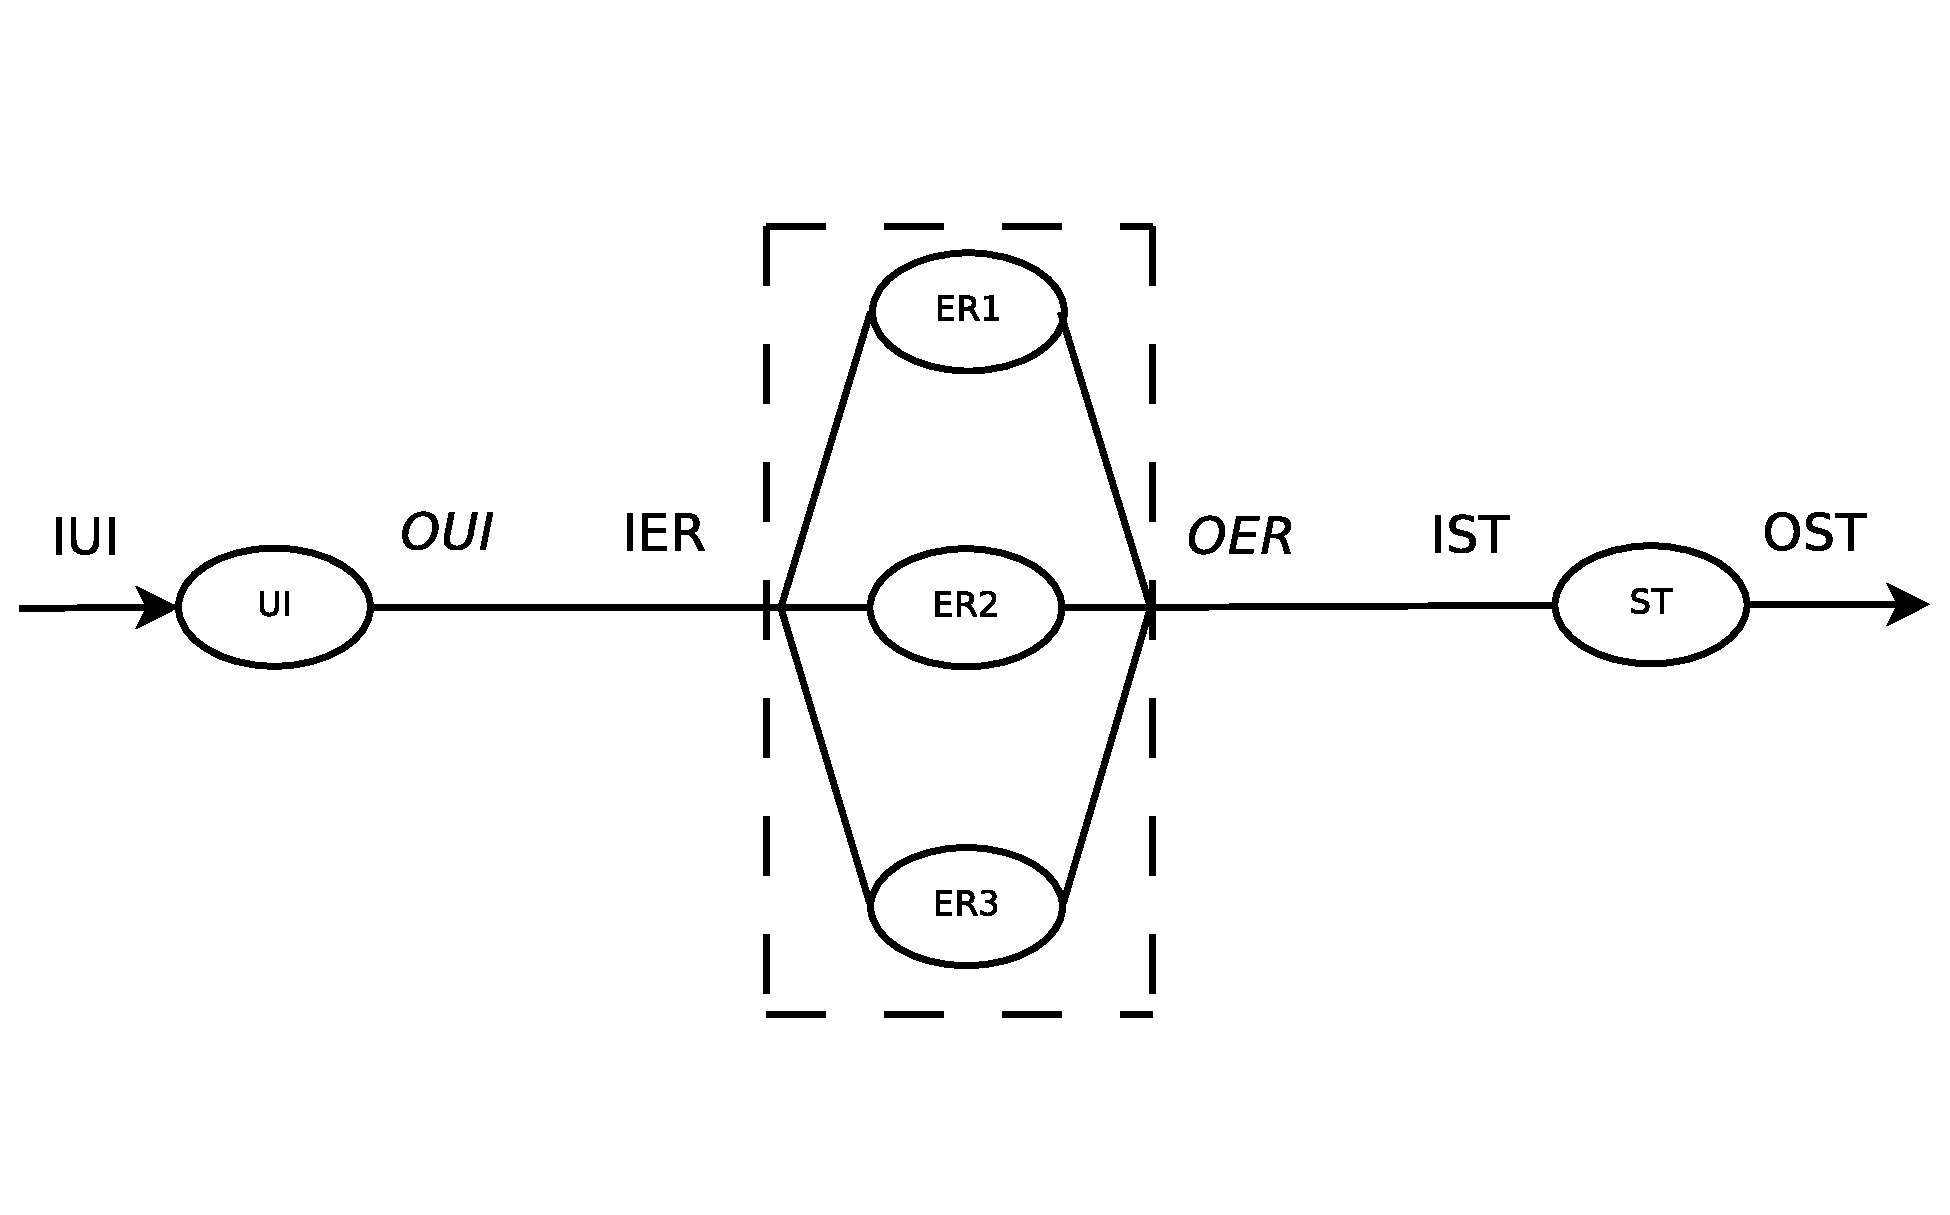
\includegraphics[width=12cm]{./states.eps}
\caption{\label{fig:events_diagram} Diagrama de estados del sistema.}
\end{center}
\end{figure}



\section{Punto (d)}
Para la simulación se utilizó el generador de numeros pseudo-aleatorios GLC de octave, utilizando como semilla el numero 1000. El tiempo de simulación se extiende hasta aproximadamente 22000 minutos, aunque se le proporcionan entradas al sistema por 50 hs. Esto se implementó de esta manera para que se otorgue un margen que permita finalizar la atención de todas las unidades encoladas. Los resultados obtenidos para la longitud de la cola en UI se pueden ver en la Figura \ref{fig:cola_UI}. Como podemos ver, al inicio de la simulación, la misma aumenta de forma casi lineal llegando a un máximo de aproximadamente 180 unidades en la cola. Luego de este punto comienza el descenso, que coincide con el instante en el cual se dejan de ingresar unidades al sistema. Este comportamiento es esperado, ya que dado que el tiempo de atención de la UI tiene una distribución uniforme entre 10 y 20 (minutos), se presenta un cuello de botella en este punto. Esto sucede porque la entrada tiene distribución exponencial con media $8.2202$ minutos.\\
\begin{figure}[ht]
\begin{center}
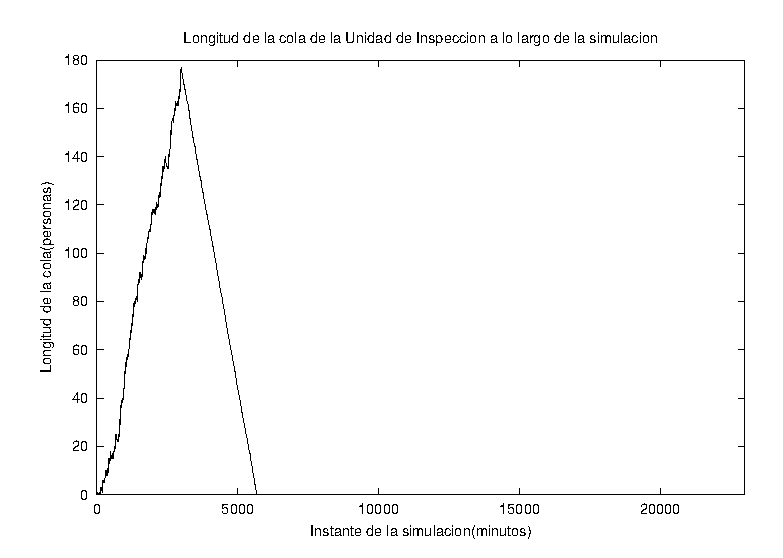
\includegraphics[width=15cm]{./img/cola_UI.eps}
\caption{\label{fig:cola_UI} Longitud de la cola de la Unidad de Inspecci\'on a lo largo de la simulaci\'on.}
\end{center}
\end{figure}
En la Figura \ref{fig:cola_ER} podemos ver la longitud de la cola de ER durante la simulación. Como el tiempo de atención tiene distribución gaussiana con media 1.05, es esperable que la longitud de la cola se mantenga en 0 permanentemente, ya que apenas sale una unidad de UI, alguno de los servidores de ER ya esta disponible para atenderlo.\\

\begin{figure}[ht]
\begin{center}
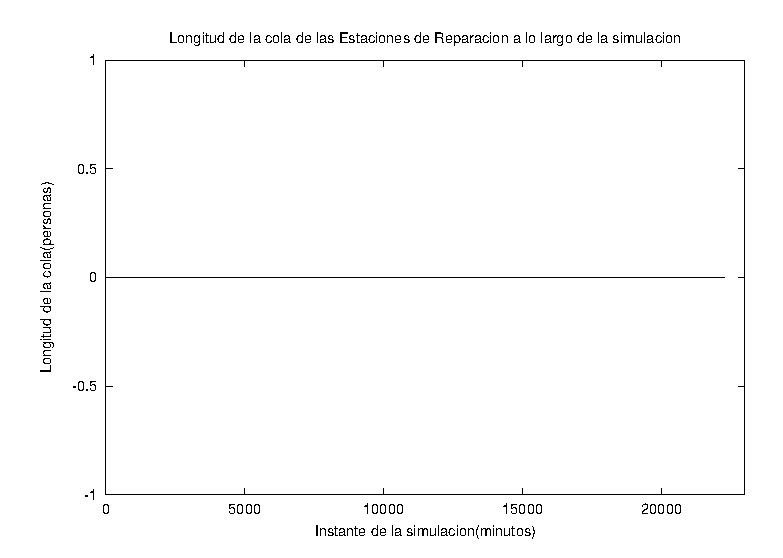
\includegraphics[width=15cm]{./img/cola_ER.eps}
\caption{\label{fig:cola_ER} Longitud de la cola de las Estaciones de Reparaci\'on a lo largo de la simulaci\'on.}
\end{center}
\end{figure}
Por último, podemos ver la Figura \ref{fig:cola_ST} que nos muestra la longitud de la cola de ST durante toda la simulación. Podemos ver que se comporta también de una forma aproximadamente lineal, aumentando mientras existen ingresos al sistema y comenzando su descenso apenas se detienen los mismos.
\begin{figure}[ht]
\begin{center}
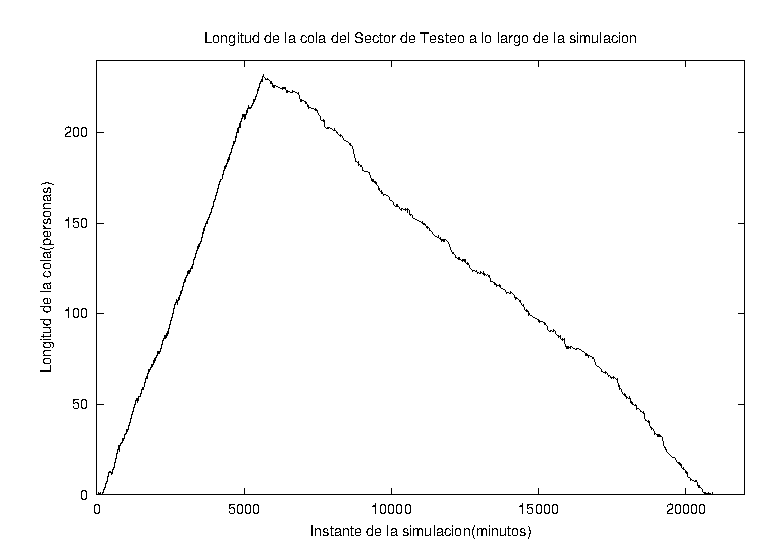
\includegraphics[width=15cm]{./img/cola_ST.eps}
\caption{\label{fig:cola_ST} Longitud de la cola del Sector de Testeo a lo largo de la simulaci\'on.}
\end{center}
\end{figure}

\section{Punto (e)}

\begin{table}
\centering
\begin{tabular}{|c|c|}
\hline
  N\'umero de simulaci\'on & Tiempo medio por cliente en el sistema(minutos) \\
\hline
  1 & 8020 \\
\hline
  2 & 8192.51 \\
\hline
  3 & 8507.83 \\
\hline
  4 & 7110.46 \\
\hline
  5 & 7853.66 \\
\hline
  6 & 8324.77 \\
\hline
  7 & 7052.01 \\
\hline
  8 & 7569.09 \\
\hline
  9 & 8831.43 \\
\hline
  10 & 7815.52 \\
\hline
\end{tabular}
\caption{\label{tab:mean_sistem_time} Tiempo medio del cliente en el sistema para distintas simulaciones}
\end{table} 
A partir de la realización de 10 simulaciónes de 50 hs cada una, se obtuvieron las estimaciónes presentadas en la tabla \ref{tab:mean_sistem_time} y la mostrada a continuación.\\
Estimaci\'on del tiempo medio por cliente en el sistema: $7927.73 /pm 1592$ con un nivel de significaci\'on del 5\%.


\section{Punto (f)}

\begin{figure}[ht]
\begin{center}
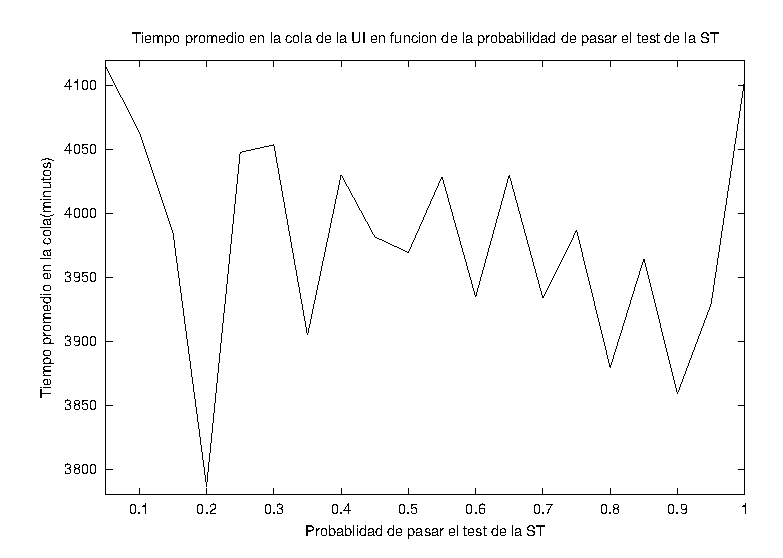
\includegraphics[width=15cm]{./img/tp_UI.eps}
\caption{\label{fig:tp_UI} Tiempo promedio en la cola de la Unidad de Inspecci\'on en funci\'on de la probabilidad de pasar el test del Sector de Testeo.}
\end{center}
\end{figure}

\begin{figure}[ht]
\begin{center}
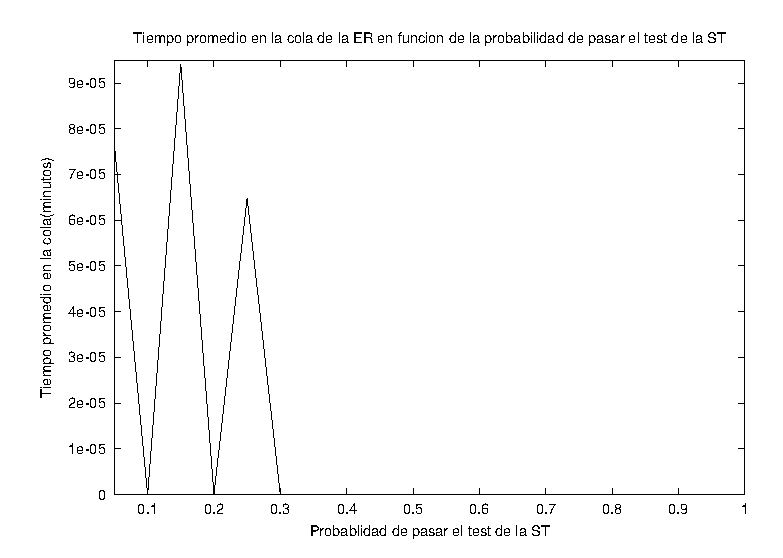
\includegraphics[width=15cm]{./img/tp_ER.eps}
\caption{\label{fig:tp_ER} Tiempo promedio en la cola de las Estaciones de Reparaci\'on en funci\'on de la probabilidad de pasar el test del Sector de Testeo.}
\end{center}
\end{figure}

\begin{figure}[ht]
\begin{center}
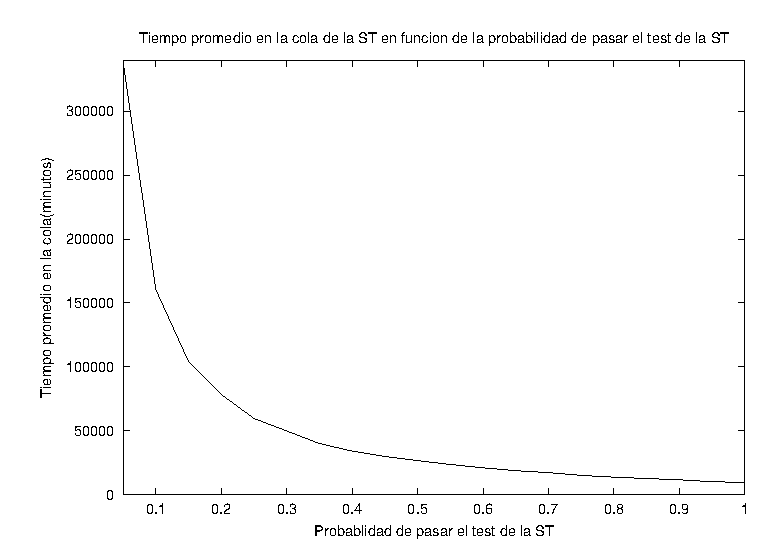
\includegraphics[width=15cm]{./img/tp_ST.eps}
\caption{\label{fig:tp_ST} Tiempo promedio en la cola del Sector de Testeo en funci\'on de la probabilidad de pasar el test del Sector de Testeo.}
\end{center}
\end{figure}

\begin{figure}[ht]
\begin{center}
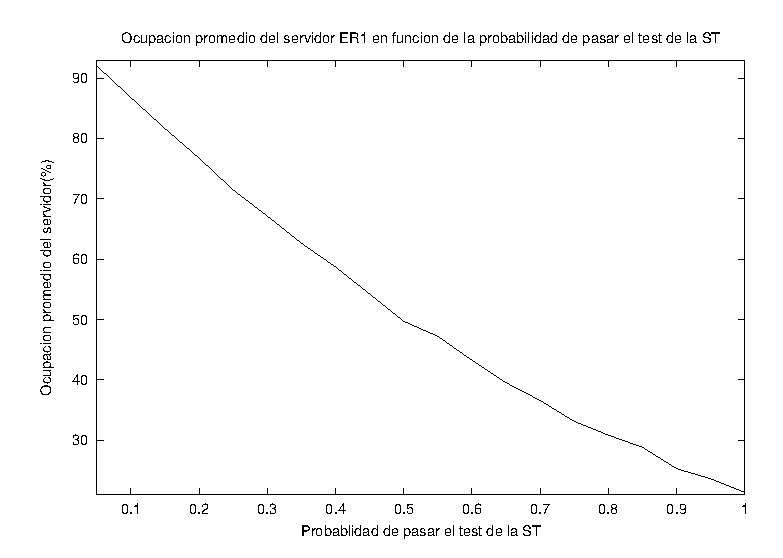
\includegraphics[width=15cm]{./img/ss_ER1.eps}
\caption{\label{fig:ss_ER1} Ocupaci\'on promedio de la Estaci\'on de Reparaci\'on 1 en funci\'on de la probabilidad de pasar el test del Sector de Testeo.}
\end{center}
\end{figure}

\begin{figure}[ht]
\begin{center}
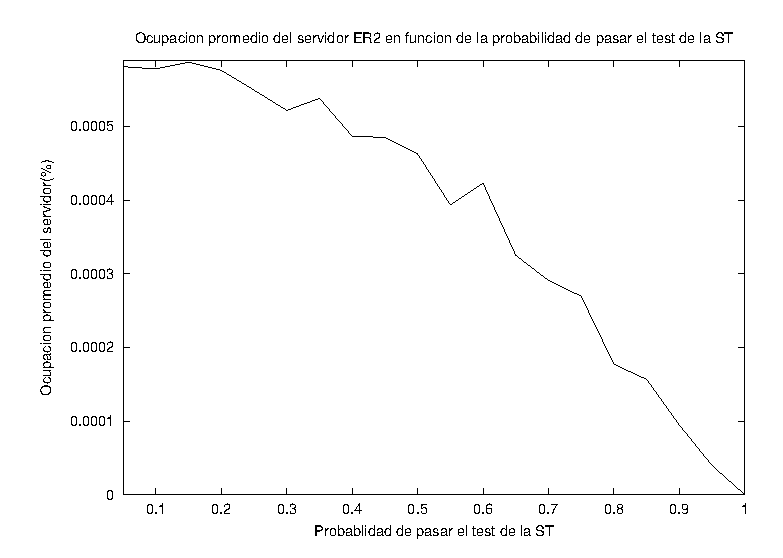
\includegraphics[width=15cm]{./img/ss_ER2.eps}
\caption{\label{fig:ss_ER2} Ocupaci\'on promedio de la Estaci\'on de Reparaci\'on 2 en funci\'on de la probabilidad de pasar el test del Sector de Testeo.}
\end{center}
\end{figure}

\begin{figure}[ht]
\begin{center}
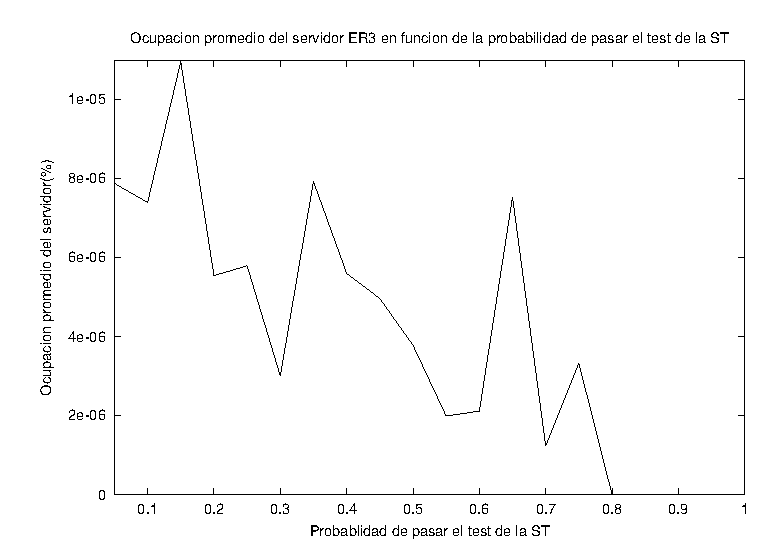
\includegraphics[width=15cm]{./img/ss_ER3.eps}
\caption{\label{fig:ss_ER3} Ocupaci\'on promedio de la Estaci\'on de Reparaci\'on 3 en funci\'on de la probabilidad de pasar el test del Sector de Testeo.}
\end{center}
\end{figure}

\begin{figure}[ht]
\begin{center}
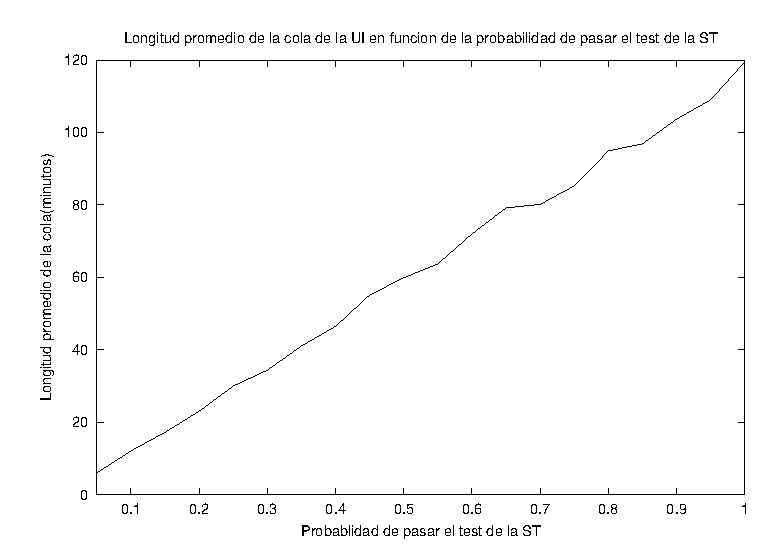
\includegraphics[width=15cm]{./img/ql_UI.eps}
\caption{\label{fig:ql_UI} Longitud promedio de la cola de la Unidad de Inspecci\'on en funci\'on de la probabilidad de pasar el test del Sector de Testeo.}
\end{center}
\end{figure}

\begin{figure}[ht]
\begin{center}
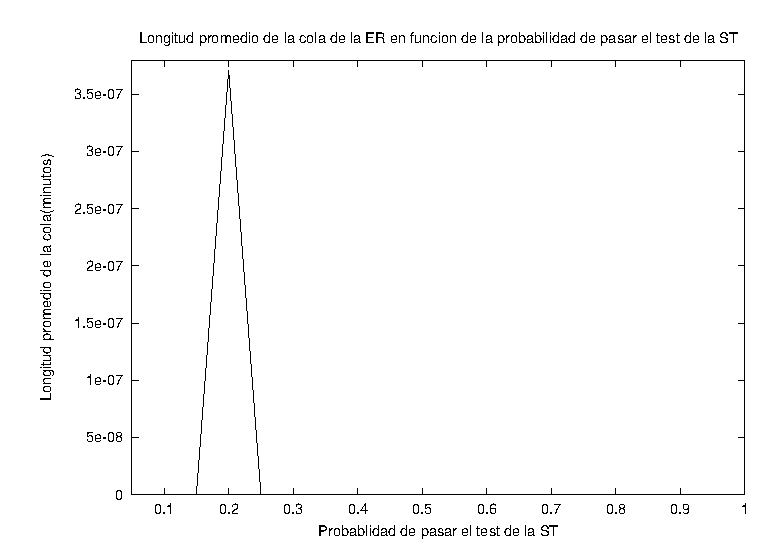
\includegraphics[width=15cm]{./img/ql_ER.eps}
\caption{\label{fig:ql_ER} Longitud promedio de la cola de las Estaciones de Reparaci\'on en funci\'on de la probabilidad de pasar el test del Sector de Testeo.}
\end{center}
\end{figure}

\begin{figure}[ht]
\begin{center}
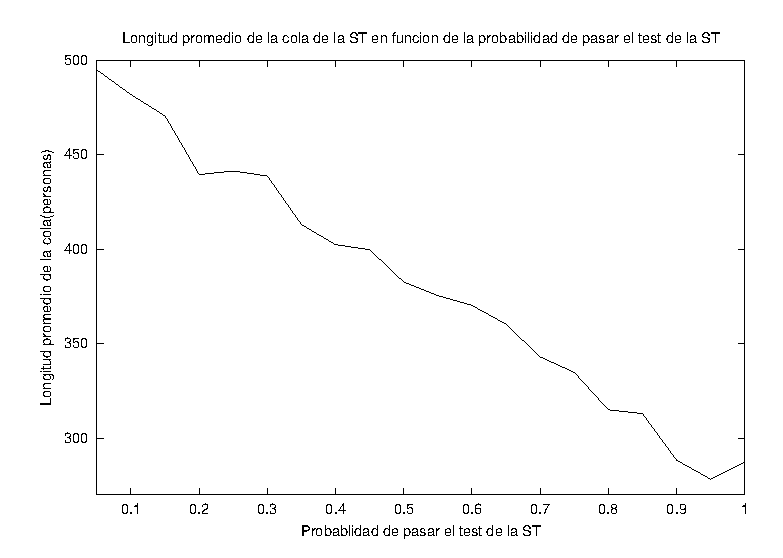
\includegraphics[width=15cm]{./img/ql_ST.eps}
\caption{\label{fig:ql_ST} Longitud promedio de la cola del Sector de Testeo en funci\'on de la probabilidad de pasar el test del Sector de Testeo.}
\end{center}
\end{figure}

\begin{thebibliography}{10}
\bibitem{chiTable} Tabla $\chi^{2}$.
\begin{verbatim}
http://www.wiphala.net/research/manual/
statistic/chi_cuadrado.html
\end{verbatim}
%\bibitem{KSTable} Tabla Kolmogorov-Smirnov.
%\begin{verbatim}
%http://www.eridlc.com/onlinetextbook/
%appendix/table7.htm
%\end{verbatim}
\end{thebibliography}

\end{document}